\section{Short Introduction to Stochastic Processes}
This part will introduce the basic equations that are relevant for the handling of Brownian motion as a stochastic process (and its realisations in a computational model) and give an equivalent Fokker-Planck equation. Furthermore it will treat the fluctuating potential barrier in terms of a Master-Equation. \\
The combination of both will be used to treat the problem of reaction rates over fluctuating barrier as a system of coupled partial differential equations that can be used to derive an analytic expression for the wanted density profiles and reaction rates.
\subsection{The Fokker Planck Equation}
\label{fpeq}
Brownian motion is a markovian process, i.e. each time step in the random motion of particles does only depend on their preceding position. This implies, that the conditional probability density function (pdf) of their coordinates obeys the following relation:
\begin{equation}
    p(x_{3},t_{3}|x_{2},t_{2};x_{1},t_{1}) = p(x_{3},t_{3}|x_{2},t_{2}), \quad t_{3}>t_{2}>t_{1}
    \label{}
\end{equation}
This relation implies, that for a Markov process every multi step probability distribution can be expressed as a hierarchy of a initial distribution and the two step transition probabilities. For $ t_1 < t_2 < \cdots < t_n$:
\begin{align}
    p(x_1,t_1;x_2,t_2;\cdots;x_n,t_n) &= p(x_n,t_n|x_{n-1},t_{n-1})P(x_{n-1},t_{n-1}|x_{n-2},t_{n-2}) \cdots \nonumber \\
                                      & \cdots p(x_2,t_2|x_1,t_1)p(x_1,t_1)
    \label{hierarchy}
\end{align}
So the entire realization of the process is determined by the initial distribution and the two step transition probability. \\
Integrating the three step joint probability distribution over the intermediate step leads to the Chapman Kolmogorov equation
\begin{equation}
    p(x_3,t_3|x_1,t_1) = \int p(x_3,t_3|x_2,t_2) p(x_2,t_2|x_1,t_1) {\rm d} x_2.
    \label{Chapman Kolmogorov equation}
\end{equation}
From the Chapman Kolmogorov equation we will derive the Kramers Moyal expansion. Therefore we multiply  with $p(x_1,t_1)$ and integrating over $x_1$ which leads to
\begin{equation}
    p(x_3,t_3) = \int p(x_3,t_3|x_2,t_2)p(x_2,t_2) {\rm d} x_2.
    \label{ck3}
\end{equation}
The integrand may be written in terms of $\Delta x = x_3 - x_2$ and then be expanded for $\Delta x << 1$
\begin{align}
    p(x_3,t_3|x_2,t_2)p(x_2,t_2) &= p( (x_3 - \Delta x) + \Delta x, t_3|x_3 - \Delta x, t_2)p( (x_3 - \Delta x), t_2) \nonumber \\
    &= \sum_{n=0}^{\infty} \frac{(-1)_{n}}{n!}\frac{\partial^{n}}{\partial x_3^{n}}\left\{p(x_3 + \Delta x, t_3|x_3,t_2) p(x_3,t_2)\right\}
\end{align}
Inserting again in \eqref{ck3} integrating over $\Delta x$ and substituting $\Delta t = t_3 - t_2$ yields
\begin{equation}
    p(x_3,t_2 + \Delta t) = \sum_{n=0}^{\infty} \frac{(-1)_{n}}{n!}\frac{\partial^{n}}{\partial x_3^{n}}\left\{ M_{n}(x_3,t,\Delta t) p(x_3,t_2) \right\}
    \label{KM1}
\end{equation}
where $M_n$ are the so called \textit{jump moments} defined by
\begin{equation}
    M_n(x,t,\Delta t) = \int (\Delta x)^{n} p(x + \Delta x, t + \Delta t | x, t) {\rm d} (\Delta x).
    \label{Jump_moments}
\end{equation}
Since $p(x+\Delta x, t|x,t) = \delta (\Delta x)$ it follows from the definition of the jump moments, that $\lim_{\Delta t \rightarrow 0} M_{n}(x,t,\Delta t) = 0$ for $n > 1$. Also $M_{0}(x,t,\Delta t) = 1$. Bearing this in mind, we now assume, that the jump moments can be expanded for $n > 1$ and small $\Delta t$
\begin{equation}
    M_{n}(x,t,\Delta t) = K^{(n)}(x,t)\Delta t + O(\Delta t^{2}).
\end{equation}
Substituting this into equation \eqref{KM1}, dividing by $\Delta t$ and taking the limit $\Delta t \rightarrow 0$ results in 
\begin{equation}
    \frac{\partial p(x,t)}{\partial t} = \sum_{n = 1}^{\infty}\frac{(-1)^{n}}{n!}\frac{\partial^n}{\partial x^n} \left\{ K^{(m)}(x,t) p(x,t) \right\}.
    \label{Kramers Moyal expansion}
\end{equation}
The so called Kramers-Moyal coefficients $K_{n}(x,t)$ can be calculated from the transition probability $T_{\Delta t}(x,\Delta x,t) = p(x+\Delta x,t+\Delta t | x, t)$:
\begin{equation}
    K^{(n)}(x,t) = \lim_{\Delta t \rightarrow 0} \frac{1}{\Delta t} \int {\rm d}(\Delta x) T_{\Delta t}(x,\Delta x,t) (\Delta x)^m .
    \label{jump moments}
\end{equation}
So far nothing has be assumed, other than the Markov property and the existence of the Taylor series. However in many application the examination of the jump moments reveals, that it is a suitable approximation to truncate the expansion for $n>2$. In this case, one obtains the following form, known as the \textit{Fokker Planck equation}   
If the expansion is truncated after the second term, the result gives the well known Fokker Planck Equation:
\begin{equation}
    \frac{\partial p(x,t)}{\partial t} = - \frac{\partial}{\partial x} \left[A(x,t)p(x,t) \right] + \frac{1}{2}\frac{\partial^2}{\partial x^2}\left[ B(x,t)p(x,t) \right] 
    \label{FPE}
\end{equation}
where $A$ and $B$ are independent of $t$ if the process is stationary. \\
\subsection{Brownian Motion}
Brownian motion is the oldest example of a Markov process that is known in physics. A heavy particle in a solution of lighter particles, which collide with it in a random fashion. Consequently, the velocity of the heavier particle undergoes a series of supposedly uncorrelated jumps. When the velocity $v$ has a certain direction, there will be on average more collisions from this side, than from the other. Therefore the probability of a change in velocity $\Delta v$ depends on its current value, but not on the velocity at earlier times. As a consequence, the velocity of the heavier particle can be considered to be a Markov process. When the whole system is in equilibrium the process is stationary and its autocorrelation time is the time in which an initial velocity is damped out. \\
Now in the \textit{overdamped limit} the correlation time of the velocity is much smaller then the time between two observations of the heavy particle. In that case the observation of the particle gives a series of positions $x(t_1), x(t_2) \cdots$. Each displacement $x(t_{i+1}) - x(t_{i})$ does not depend on the previous history of the process, i.e. it is independent of $x_{i=1}, x_{i-2}\cdots$. Hence not only the velocity, but also the position of the particle is a Markov process (at least on a coarse grained timescale). 
\par
In the following we will start with the Langewin equation for the velocity of a particle in a fluid and derive the corresponding Kramers Moyal coefficients to obtain a Fokker-Planck equation for the distribution of its position. 

\begin{equation}
    m \frac{{\rm d}^2 x}{{\rm d}t^2} = -\gamma \frac{ {\rm d}x}{{\rm d}t} + f(x) + \varepsilon(t)
    \label{Langewin equation}
\end{equation}
Here $\varepsilon(t)$ is a Gaussian distributed random process describing the collision interaction of the particle and the solute. $f(x)$ is a force resulting from an external potential and is taken to be independent of $t$. It can be shown, that the correlation time of this process is $\tau = \dfrac{m}{\gamma}$. In the so called overdamped limit $ \tau >> 1$ this equation results in
\begin{equation}
    \gamma \frac{ {\rm d}x}{{\rm d}t} = f(x) + \varepsilon(t)
    \label{BD1}
\end{equation}
As described in the introductory part the process must be observed on a coarse grained timescale to be considered Markovian. Therefore the expression can be discretized in time and transforms to:
\begin{equation}
        x(t + \Delta t) = x(t) + \frac{1}{\gamma}f(x,t) \Delta t + \frac{1}{\gamma} \varepsilon'(t) \Delta t.
    \label{overdamped limit}
\end{equation}
with the distribution of the random force being
\begin{equation}
    P(\varepsilon ' ) = \sqrt{\frac{\Delta t}{4 \pi D \gamma^{2}}} \exp \left[ - \frac{\varepsilon ^{\prime 2} \Delta t}{4 D \gamma^{2}} \right].
    \label{eps dist}
\end{equation}
From this distribution one can compute the transitions probability for the Brownian particle as:
\begin{align}
    T_{\Delta t}(x,\Delta x,t)  &= \left< \delta \left(  \Delta x - (x(t-\Delta t) - x(t)) \right)\right> \nonumber\\
                        &= \int \rm{d}\varepsilon ' \delta \left(  \Delta x - (x(t-\Delta t) - x(t)) \right)  \sqrt{\frac{\Delta t}{4 \pi D \gamma^{2}}} \exp \left[ - \frac{\varepsilon  ^{\prime 2} \Delta t}{4 D \gamma^{2}} \right] \nonumber\\
                        &= \sqrt{\frac{1}{4 \pi D \Delta t}} \exp \left[ \frac{-\left(\Delta x - f(x) \frac{\Delta t}{\gamma} \right)^2}{4 D \Delta t} \right]
    \label{T}
\end{align}
For this Gaussian transition probability the coefficients of the Kramers Moyal Expansion vanish after the second term, such that the resulting Fokker Planck equation holds the full analytic solution for the time evolution of the distribution of particles.
\begin{equation}
    \frac{\partial p(x,t)}{\partial t} = - \frac{\partial}{\partial x} \left[f(x)p(x,t) \right] + D\frac{\partial^2}{\partial x^2}\left[p(x,t) \right] 
    \label{FPE2}
\end{equation}

\subsection{The Master-Equation}
\label{meq}
The master equation is an equivalent formulation of the Fokker-Planck equation for a certain class of stochastic processes. Namely those, whose transition probability has the following behaviour in the limit of small time steps $\Delta t$:
\begin{equation}
    p(x_2,t+\Delta t|x_1,t) = W(x_2|x_1)\Delta t + \left[ 1 - \Delta t \int {\rm d} x W(x_2|x_1) \right] \delta(x_2-x_1) + O(\Delta t ^{2})
    \label{master assumption}
\end{equation}
This assumption has the following meaning: The system was in state $x_1$ at time $t$ and made a transition to state $x_2$ during the time $\Delta t$. Then the probability of the transition is expressed in terms of the (non negative) {\it transition rate} i.e. the transition probability per unit time $W(x_2|x_1)$. To maintain a readable form we introduce the notation $T_\tau (x_2|x_1) = p(x_2,t+\tau|x_1,t)$ and omit the absolute time dependence, since the process is assumed to be stationary. \\
Using the Chapman-Kolmogorov equation it follows that
\begin{equation}
    T_{\tau + \tau'}(x_3|x_2) = \int T_{\tau'}(x_3|x_2)T_{\tau}(x_2|x_1){\rm d} x_2,
    \label{K2}
\end{equation}
and thus:
\begin{equation*}
    T_{\tau+\tau'}(x_3|x_1) = \int \left\{ \left[1 - \tau' \int {\rm d} z W(z|x_3) \right] \delta(x_3 - x_2) + \tau' W(x_3|x_2) \right\} T_{\tau}(x_2|x_1){\rm d} x_2
\end{equation*}
Regrouping the terms and dividing by $\tau ' $ leads to:
\begin{align*}
    \frac{1}{\tau'} T_{\tau+\tau'}(x_3|x_1) &= \frac{1}{\tau'}  \int T_{\tau}(x_2|x_1) \delta(x_3 - x_2){\rm d} x_2\\
    &- \int \left\{ W(z|x_2)  T_{\tau}(x_2|x_1)\delta(x_3 - x_2) \right\}{\rm d} z {\rm d} x_2 \\
    &+ \int \left\{ W(x_3|x_2) T_{\tau}(x_2|x_1) \right\}{\rm d} x_2
\end{align*}
which in the limit of $\tau' \rightarrow 0$ leads to the desired master equation:
\begin{equation}
    \frac{\partial}{\partial \tau}T_{\tau}(x_3|x_1) = \int \left\{ W(x_3|x_2) T_{\tau}(x_2|x_1) - W(x_2|x_3) T_{\tau}(x_3|x_1) \right\}{\rm d} x_2
    \label{continuous_space_master_equation}
\end{equation}
where the $W(x_i|x_j)$ are properties of the specific process.
This equation describes the time development of the transition probabilities given an initial condition $(x_1,t_1)$. A more intuitive form follows from multiplying and integrating over a distribution of initial conditions $p(x_1,t_1)$ and its spatial coordinate $x_1$.
\begin{equation}
    \frac{\partial p(x,t)}{\partial t} = \int \left\{ W(x|x') p(x',t) - W(x'|x)p(x,t) \right\} {\rm } x'
\end{equation}
In this form the meaning becomes particularly clear. The master equation is a \textit{gain loss equaition} for the probabilities of each state $x$. The first term on the rhs. describes the gain of probability of state $x$ due to transitions from other states $x'$, whereas the second term on the lhs. describes the loss of probability of state $x$ due to transitions to other states.\\
For a discrete state space, the master equation has the form of a system of coupled ordinary differential equations:
\begin{equation}
    \frac{{\rm d} p_n(t)}{{\rm d} t} = \sum_{n'} W_{n n'}p_{n'}(t) - W_{n'n}p_{n}(t)
    \label{discrete_space_master_equation}
\end{equation}
$W$ is called a transition rate matrix and satisfies the following conditions:
\begin{align*}
    &0 \ge W_{n,n'} \quad \mbox{ for all } n \ne n' \\
    &0 \ge -W_{n,n} \ge \infty \\
    &\sum_{n'} W_{n,n'} = 0
    \label{Transitions_rate_matrix}
\end{align*}
In general it is not symmetric and can thus not be diagonalized. \\
From eq. \eqref{discrete_space_master_equation} one immediately sees, that for a steady state solution this implies, that the loss of probability from one state is compensated by the gain of probability by transitions from other states.\\
For stationary time reversible Markov processes this criterion can even be tightened to a property called \textit{detailed equilibrium}.
This property requires, that the total amount of probability going from two states in to each other must be equal i.e.
\begin{equation}
     W_{n n'}p_{n'} = W_{n'n}p_{n}
    \label{detailed_balance}
\end{equation}
This property implies a certain symmetry of the matrix and can be used to show, that for this class of transition rate matrices can be transformed to a symmetric state such that they can be diagonalized via a suitable orthogonal transformation.
\subsection{Multivariate Markov Processes}
It is straight forward to continue to Markov processes whose sample space is a direct product of continuous and discrete variables i.e. $\Omega = \mathbb{R}^{3} \times [1,\cdots, N]$. The Chapman Kolmogorov equation then becomes
\begin{equation}
    p(\vec{x}_3,n_3,t_3|\vec{x}_1,n_1,t_1) = \sum_{n_2} \int p(\vec{x}_3,n_3,t_1|\vec{x}_2,n_2,t_2)p(\vec{x}_2,n_2,t_2|\vec{x}_1,n_1,t_1) {\rm d} \vec{x}_2
    \label{MCK}
\end{equation}
In this case the variable $\vec{x}$ can be treated by the approach discussed in section \ref{fpeq} whereas the variable $n$ will be treated by the approach described in section \ref{meq}. This leads to a combined Master Fokker-Planck equation for the time evolution of the pdf
\begin{align}
    \frac{\partial}{\partial t } p(\vec{x},n,t) =   &- \vec{ \nabla } \left[\vec{A}(\vec{x},n,t)p(\vec{x},n,t) \right] + \frac{1}{2}\vec{\nabla}^{2}\left[ B(\vec{x},n,t)p(\vec{x},n,t) \right] \nonumber \\
                                                    &+ \sum_{n'} \left\{ W_{nn'}p(\vec{x},n',t) - W_{n'n}p(\vec{x},n,t)\right\}
    \label{fpmeq1}
\end{align}
It is convenient to write this equation in a vector notation for the variable $n$ indicating with $\vect{p}$ the vector $(p(0),p(1),\cdots,p(N))$ the vector on the $N$ dimensional space over the closed interval $[0,1]$ (the variables $\vect{x}$ and $t$ have been omitted). \\ 
Therefore we introduce a diagonal Fokker-Planck operator for the drift and diffusion terms
\begin{equation}
    \mathbb{F} = - \vec{ \nabla } \vec{A}(\vec{x},n,t) + \frac{1}{2}\vec{\nabla}^{2} B(\vec{x},n,t)
    \label{fpo}
\end{equation}
and write the transition rate matrix as $\mathbb{W}$ as
\begin{align*}
    &\mathbb{W}_{n,n'} = W_{nn'} \mbox{ for } n \ne n' \mbox{ as in eq. \eqref{discrete_space_master_equation}} \\
    &\mathbb{W}_{nn} = -\sum_{n \ne n'}W_{nn'}
\end{align*}
such that eq. \eqref{fpmeq1} has the following more compact form
\begin{equation}
    \frac{\partial}{\partial t} \vect{p}(\vec{x},t) = \left\{ \mathbb{F} + \mathbb{W} \right\} \vect{p}(\vec{x},t).
    \label{fpmeq2}
\end{equation}

\section{The Debye Reaction Rate}
For educational reasons and since we will refer to it later, we will at this point give the solution to the original Debye problem.
The problem involves a perfect spherical of radius $R_s$ sink embedded in an initially homogeneous distribution of Brownian particles. The aim is to calculate the time dependent and stationary absorption rate of particles into the sink.
The boundary and initial conditions are therefore
\begin{align}
    \rho(r > R_s, t = 0) &= \rho_o, \\
    \rho(r=R_s,t) &= 0, \\
    \lim_{r \rightarrow \infty} \rho(r, t) &= \rho_o.
    \label{BC}
\end{align}
In the following, the corresponding Fokker Planck Equation in terms of particle densities
\begin{equation}
        \frac{\partial \rho(\vec{r},t)}{\partial t} = - \vec \nabla \left[ \vec f(\vec{r})\rho(\vec{r},t) \right] + D\vec \nabla ^2 \left[\rho(\vec{r},t) \right] 
    \label{FPE3}
\end{equation}
will be solved without external force, i.e. $\vec f(r) = 0$ and subject to the given boundary and initial conditions.
With the substitution $r \cdot \rho(r,t) = u(r,t)$ and the assumption, that the problem is spherically symmetric the derivatives in the Fokker Planck equation simplify to
\begin{equation}
    \frac{\partial u(r,t)}{\partial t} = D \frac{\partial ^2 u(r,t)}{\partial r^2}
    \label{Simplified FPE}
\end{equation}
Laplace transform of the equation yields:
\begin{align}
    \int_0^\infty e^{-st}\frac{\partial u(r,t)}{\partial t} \rm{d} t &= D \frac{\partial ^2 }{\partial r^2} \int_0^\infty e^{-st} u(r,t) \rm{d} t \\
    \left[e^{-st} u(r,t) \right]_0^\infty + s \int_0^\infty e^{-st} u(r,t) \rm{d} t &= D \frac{\partial^2}{\partial r^2} \tilde{u}(r,s)\\
    u(r,0) + s \tilde{u}(r,s) &= D \frac{\rm{d}^2}{\rm{d} r^2} \tilde{u}(r,s).
\end{align}
This is an ordinary 2nd degree inhomogeneous differential equation with constant coefficients.
For the standard ansatz $\tilde{u}(r,s) = \exp(\lambda(s) r)$ for the homogeneous solution we get the following characteristic polynomial:
\begin{equation}
    \lambda(s) ^2 - \frac{s}{D} = 0
    \label{}
\end{equation}
resulting in the following homogeneous solution:
\begin{equation}
    \tilde{u}_h(r,s) = C_1 e^{ - \sqrt{\frac{s}{D}} \cdot r } + C_2 e^{ \sqrt{\frac{s}{D}} \cdot r }
    \label{u_h}
\end{equation}
We find the inhomogeneous solution using a polynomial ansatz of the form $\tilde{u}_i = C_3 r + C_4$ leading to the following relation:
\begin{align}
    s(C_3 r + C_4)  &= -u(r,0)\\
                    &= - r \rho_o \\
    \Rightarrow C_3 &= \frac{r}{s}\rho_o \\
                C_4 &= 0
\end{align}
Now the entire solution has to be fitted to the boundary conditions as in (\ref{BC}). The solution in Laplace space then reads:
\begin{equation}
\tilde{u}(r,s) = \rho_o \left( \frac{r}{s} + \frac{R_s}{s} e^{ \sqrt{\frac{s}{D}}(R_s - r) } \right) 
\end{equation}
The inverse Laplace transform
\begin{align}
    u(r,t)  &= \frac{1}{2 \pi i} \int\limits_{\gamma - i \infty}^{\gamma + i \infty}  e^{st} \tilde{u}(r,s){\rm d}t \\
    &= \frac{\rho_o}{ 2 \pi i} \left\{  \int\limits_{\gamma - i \infty}^{\gamma + i \infty} \frac{r}{s}  {\rm d}t +  \int\limits_{\gamma - i \infty}^{\gamma + i \infty}\frac{R_s}{s} e^{ \sqrt{\frac{s}{D}}(R_s - r) }  {\rm d}t \right\}
    \label{inverse laplace}
\end{align}
is done using the residue theorem for the first integral:
\begin{align}
    \oint_{ \gamma } {\rm d}z f(z) &= 2 \pi i \sum_{k = 1}^{n}I(\gamma, a_k) {\rm Res}(f,a_k) \\
    { \rm Res}(f,y_o) &= \frac{1}{(m-1)!} \lim_{z\rightarrow z_o} \frac{{ \rm d} ^{m-1}}{{\rm d} z^{m-1}} \left[ (z - z_o)^{m}f(z) \right]
    \label{residue theorem}
\end{align}
and the following identity for the second:
\begin{equation}
    \mathcal{L}\left[ {\rm erfc\left( \frac{a}{2\sqrt{t}} \right)} \right] = \frac{1}{s}e^{a\sqrt{s}}
    \label{L(erfc)}
\end{equation}
resulting in the following time dependent solution for $u(r,t)$ resp. the particle density $\rho(r,t)$:
\begin{align}
    u(r,t) &= \rho_o \left\{ r - R_s {\rm erfc} \left( \frac{r - R_s}{\sqrt{4 D t}} \right) \right\} \\
    \rho(r,t) &= \rho_o \left\{ 1 - \frac{R_s}{r} + {\rm erf} \left( \frac{r - R_s}{\sqrt{4Dt}} \right) \right\}.
    \label{u(r,t)}
\end{align}
In the limit $t \leftarrow \infty$ this results in the steady state density profile:
\begin{equation}
    \rho(r) =  \rho_o \left( 1 - \frac{R_s}{r} \right)
    \label{steady state density}
\end{equation}
The reaction rate can be defined as the total flux of particles through the boundary $\Omega$ of the sink:
\begin{equation}
    K = \int_\Omega \vec{J} {\rm d}\vec{A} 
    \label{reaction rate}
\end{equation}
Using the differential continuity equation:
\begin{align}
    \frac{\partial \rho(\vec{r},t)}{\partial t}&= \vec{\nabla} \vec{J}(\vec{r},t) \\
    &= \vec{\nabla} \left\{ \rho(\vec{r},t) \nabla \vec{U}(\vec{r}) + D \vec{\nabla} \rho(\vec{r},t) \right\}
    \label{contiuity equation}
\end{align}
and the spherical symmetry of the solution one can derive the time dependent reaction rate of the Brownian particles with the spherical sink of radius $R_s$ as follows:
\begin{align}
    K(t) &= \int_\Omega D  \vec{\nabla} \rho(\vec{r},t) \\
    &= 4 \pi D R_s^2 \left. \vec{\nabla} \rho(\vec{r},t) \right|_{r = R_s}\\
    &= 4 \pi D R_s \rho_o \left( 1 + \frac{R_s}{\sqrt{4Dt}} \right)
    \label{ideal reaction rate}
\end{align}
Again in the limit of $t \rightarrow \infty$ this results in the steady state absorption rate:
\begin{equation}
    K = 4 \pi D R_s \rho_o
    \label{steady state ideal rate}
\end{equation}


\section{Reaction Rates over Fluctuating Barriers}
\subsection{Model Description}
The system under consideration consists of a spherical sink of radius $R_s$ that is surrounded by a potential barrier. The barrier is assumed to be of boxcar shape with limiting radius $a,b>R_s$. It fluctuates between states $n$ with different hight $U_n \in [U_0, \cdots U_N]$ subject to a transition rate matrix $\mathbb{W}$. The system is embedded in a reservoir of Brownian particles. It is desired to find the rate at which the particles are absorbed by the sink, given that the transition rate matrix of the potential fluctuations satisfies the detailed balance property.\\
The appropriate boundary conditions are, that the probability density function of the Brownian particles is zero at $R_s$ and takes a constant finite value for $|\vec{r}| \rightarrow \infty$. Due to the fact that the system is not spatially bounded it is not possible to normalize the joint pdf $\vect{p}(\vec{r},n,t)$ of the position of the Brownian particles and the state of the potential barrier in the sense that 
\begin{equation}
    \sum_n \int_{\mathbb{R}^{3}} p_n(\vec{r},t) {\rm d}V = 1.
    \label{pdfNormalization}
\end{equation}
Instead it is appropriate to normalize the distribution to the particle density $\vect{\rho}(\vec{r},t)$ as commonly done in statistical physics
\begin{equation}
    \sum_n \int_V \rho_n(\vec{r},t) {\rm d}V = N
    \label{densNormalisation}
\end{equation}
where $N$ is the total number of particles enclosed in the volume $V$. The time evolution of the joint pdf can be described by eq. \eqref{fpmeq2} derived in the previous section
\begin{equation}
    \frac{\partial}{\partial t}\vect{\rho}(\vec{r},n,t) = \left\{ \mathbb{F} + \mathbb{W} \right\} \vect{\rho}(\vec{r},n,t).
    \label{fpmeq3}
\end{equation}
Using the spherical symmetry of the system, the Fokker-Planck operator can be written as
\begin{equation}
    \mathbb{F} = {\rm diag}\left[ \vec{\nabla}\frac{1}{\gamma}\left( \vec{\nabla} U_n(r) \right)+ D \vec{\nabla}^{2} \right].
    \label{fpo2}
\end{equation}
It becomes obvious from this equation, that the state of the potential might as well be seen as a property of the Brownian particles. One could for instance imagine the barrier as a constant electric potential. Then the particles are fluctuating between differently charged states. For the assumption of noninteracting particles to be still valid, the solution has to be dilute and the Debye screening length has to be small. \\
\subsection{Fit Conditions}
For the boundary at $|\vec{r}| \rightarrow \infty$ far away from the influence of the potential and the sink it is reasonable to assume that the particle density distribution is a stationary solution $\vect{\rho}^{(eq)}$ the sole Master equation. From the assumption of detailed balance it follows that it has to satisfy
\begin{align}
    &\mathbb{W} \vect{\rho}^{(eq)} = 0 \nonumber \\
    &\mathbb{W}_{n'n} \rho_n^{(eq)} = \mathbb{W}_{nn'}\rho_{n'}^{(eq)}.
    \label{detailed_balance2}
\end{align}
It can be shown that this $\vect{\rho}^{(eq)}$ is not degenerate and that all its entries are positive. \\
The next issue to investigate is the behaviour of the steady state solution for the particle density distribution at the jump discontinuities of the potential 
\begin{equation}
  U_n(r) = \left\{ \begin{array}{l l} 
        0 &: R_s < r \le a \\
        U_n &: a<r \le b \\
        0 &: b < r \le R_d
    \end{array} \right.
    \label{step_potential}
\end{equation}
Therefore we first integrate from the boundary of the sink to some arbitrary $r > R_s$
\begin{equation*}
    \int_{R_s}^{r}\mathbb{F}\vect{\rho}(r'){\rm d} r' = - \mathbb{W} \int_{R_s}^{r} \vect{\rho}(r') {\rm d} r' .
\end{equation*}
Note that the lower boundary of the Integral on the lhs is proportional to the particle flux through the sink boundary whereas the upper bound is proportional to the particle flux through the surface of a sphere with radius $r$ at a certain state of the potential. The Integral on the rhs is proportional to the particle flux from and to the this state of the potential in the observed volume due to transitions from and to other states of the potential.\\
    \begin{equation}
        \frac{1}{\gamma}\rho_n(r) \vec{\nabla} U_n(r) + D \vec{\nabla} \rho_n(r) = J_n(R_s) - \left\{ \mathbb{W} \int_{R_s}^{r} \vect{\rho}(r') {\rm d} r' \right\}_{n}
    \end{equation}
Now we integrate over a small vicinity of the jump discontinuity with width $\varepsilon$ and take the limit of $\varepsilon \rightarrow 0$
    \begin{equation}
        \int_{a-\varepsilon}^{a + \varepsilon} \frac{U_n}{\gamma D}\delta(a-r) + \int_{a-\varepsilon}^{a + \varepsilon} \frac{1}{\rho_n(r)}\nabla \rho_n(r) = \underbrace{\int_{a - \varepsilon}^{a + \varepsilon}\frac{J_n(r)}{\rho_n(r) D} - \int_{a - \varepsilon} ^{a+ \varepsilon} \left\{ \mathbb{W} \vect{\rho}(r)\right\}_{n}}_\text{$O(\varepsilon)$}
    \end{equation}
Since the terms on the rhs. of the equation scale only with $\varepsilon$ we end up with a result previously known for systems in thermal equilibrium:
\begin{equation}
    \vect{\rho}^{(I)}(a) = \underbrace{ {\rm diag}\left[\exp\left\{\frac{U_n}{K_B T} \right\}\right]}_\text{\large$\mathbb{U}$} \vect{\rho}^{(II)}(a)
\end{equation}
Here $\vect{\rho}^{(I)}$ and $\vect{\rho}^{(II)}$ refers to the particle density at different side of the jump discontinuity.
Analogously we find relations for the derivatives of the particle density at the jump discontinuity:
\begin{equation}
    \vec{\nabla}\vect{\rho}^{(I)}(a) = \vec{\nabla}\vect{\rho}^{(II)}(a)
\end{equation}
\subsection{Expansion in Eigenfunctions of $\mathbb{W}$}
The assumption of the detailed balance property that implies the existence of an equilibrium distribution $\vect{\rho}^{(eq)}$ allows for the definition of an operator $\mathbb{T}$
\begin{equation}
    \mathbb{T} = \delta_{n,n'} [\rho_n^{(eq)}]^{\frac{1}{2}}.
    \label{symmetrisation_transform}
\end{equation}
This is a similarity transform that symmetrises $\mathbb{W}$
\begin{equation}
    \mathbb{T}^{-1}\mathbb{W}\mathbb{T} = \mathbb{S}.
    \label{symm_rate_matrix}
\end{equation}
Using property \eqref{detailed_balance2} it follows that
\begin{align}
    \mathbb{S}_{il} &= \mathbb{T}^{-1}_{ij} \mathbb{W}_{jk} \mathbb{T}_{kl} = \sum_j \delta_{ij} [\rho^{(eq)}_i]^{-\frac{1}{2}} \mathbb{W}_{jk} \mathbb{T}_{kl} \\ \nonumber
    &= [\rho^{(eq)}_{i}]^{\frac{1}{2}} \sum_{k} \mathbb{W}_{ik} \delta_{kl} [\rho^{(eq)}_l]^{-\frac{1}{2}} = \mathbb{W}_{il}^{\frac{1}{2}} \left( \mathbb{W}_{il} \frac{\rho^{(eq)}_i}{\rho^{(eq)}_l} \right)^{\frac{1}{2}} \\ \nonumber
    &= \left(\mathbb{W}_{il} \mathbb{W}_{li}\right)^{\frac{1}{2}} \\ \nonumber
    S_{ii} &= W_{ii}.
\end{align}
The resulting matrix can then be diagonalized by an orthogonal matrix $\mathbb{D}$
\begin{equation}
    \mathbb{D}^{\dagger} \mathbb{S} \mathbb{D} = -{\rm diag}\left[ \lambda_i \right].
    \label{orthogonal_transform}
\end{equation}
It can be shown that $\lambda_i > 0$ for $i>1$ and $\lambda_1 = 0$ with the corresponding eigenvector
\begin{equation}
    D_{i1} = \rho^{(eq)}(i)^{\frac{1}{2}}.
\end{equation}
We now write equation \eqref{fpmeq3} in terms of eigenfunctions of $\mathbb{W}$
\begin{equation}
    \tilde{\vect{\rho}}(\vec{r},t) = \mathbb{A}^{-1} \vect{\rho}(\vec{r},t)
    \label{eigenfunctions}
\end{equation}
where $\mathbb{A}$ denotes the transformation $\mathbb{T}\mathbb{D}$ and use the fact that the potential term vanishes everywhere but at the jump discontinuities. Therefore equation \eqref{fpmeq3} reads
\begin{equation}
    \frac{\partial }{\partial t} \tilde{\vect{\rho}}^{(j)}(\vec{r},t) = {\rm diag} \left[D \vec{\nabla}^{2} - \lambda_i  \right] \tilde{\vect{\rho}}^{(j)}(\vec{r},t)
    \label{fpmeq4}
\end{equation}
For the steady state case where the lhs. vanishes it it straight forward to write down the solution to this equation
\begin{align}
    \tilde{\rho}_{1}^{(j)}(r) &= c_{1,1}^{(j)} + c_{1,2}^{(j)} \frac{1}{r} \nonumber \\
    \tilde{\rho}_{i \ne 1}^{(j)}(r) &= c_{i,1}^{j}\frac{1}{r} \exp\left[-r\sqrt{\frac{\lambda_i}{D}}\right] + c_{i,2}^{j}\frac{1}{r} \exp\left[r\sqrt{\frac{\lambda_i}{D}}\right] 
    \label{fp_ind_sol}
\end{align}
\subsection{Treatment of Boundary and Fit Conditions}
\label{FBC}
Now we have to find an expression, that allows for the calculation of the coefficients $c_{i,k}^{(j)}$ from the transformed boundary and fit conditions
\begin{align}
    \mathbb{A}^{-1}\vect{\rho}^{(I)}(R_s) &= \vect{\tilde{\rho}}^{(I)}(R_s) = 0 \nonumber \\
    \vect{\tilde{\rho}}(r \rightarrow \infty) &= \mathbb{A}^{-1} \vect{\rho}^{(eq)} = (1,0,\cdots,0)^{T}
\end{align}
and
\begin{align}
    \vect{\tilde{\rho}}^{(I)}(a) &= \mathbb{A}^{-1}\mathbb{U}\mathbb{A} \vect{\tilde{\rho}}^{(II)}(a), \\ \nonumber
    \vect{\tilde{\rho} '}^{(I)}(a) &= \vect{\tilde{\rho} '}^{(II)}(a), \\ \nonumber
    \vect{\tilde{\rho}}^{(III)}(b) &= \mathbb{A}^{-1}\mathbb{U}\mathbb{A} \vect{\tilde{\rho}}^{(II)}(b), \\ \nonumber
    \vect{\tilde{\rho} '}^{(III)}(b) &= \vect{\tilde{\rho} '}^{(II)}(b).
\end{align}
Therefore it is useful to write the solution of eq. \eqref{fpmeq4} as
\begin{equation}
    \tilde{\vect{\rho}}^{(j)} = \underbrace{ \left( \begin{array}{cllllllll}
       1   & \frac{1}{r}   & 0                 & 0                 & 0              & 0             & 0 & \cdots &\\
       0   & 0             &\frac{1}{r} e^{-r \alpha_2}   &\frac{1}{r} e^{r \alpha_2 }   & 0              & 0             & 0 & \cdots &\\
       0   & 0             & 0                 & 0                 &\frac{1}{r} e^{-r\alpha_3} &\frac{1}{r} e^{r\alpha_3} & 0 & \cdots &\\
       \vdots  &&&&&&&\ddots &\\
       \vdots  &&&&&&&&\ddots
   \end{array} \right)}_\text{\large$\hat{\rho}(r)$}
   \underbrace{\left(\begin{array}{c}  
       c_{1,1}^{(j)} \\ 
       c_{1,2}^{(j)} \\ 
       c_{2,1}^{(j)} \\ 
       c_{2,2}^{(j)}  \\ 
       \vdots 
   \end{array} \right)}_\text{\large$\mathbb{C}$}.
\end{equation}
Here $\alpha_i = (\lambda_i / D)^{1/2}$. Using this notation, the boundary and fit conditions can be but in one $6 N$ dimensional system of linear equations
\begin{equation}
    \left( \begin{array}{lll}
        \hat{\rho}(R_s) & 0 & 0 \\
        \hat{\rho}(a)   & -\tilde{\mathbb{U}}\hat{\rho}(a) & 0 \\
        \hat{\rho}'(a) & -\hat{\rho}'(a) & 0 \\
        0 &  -\tilde{\mathbb{U}}\hat{\rho}(b) & \hat{\rho}(b) \\
        0 &  -\hat{\rho}'(a) & - \hat{\rho}'(a) \\
        0 & 0 & \hat{\rho}(r\rightarrow \infty)
    \end{array}\right) \left( \begin{array}{c} c_{1,1}^{1} \\ \vdots \\ \vdots \\ \vdots \\ c_{N,2}^{3} \end{array} \right) = 
    \left( \begin{array}{c} 0 \\ \vdots \\ 0 \\ 1 \\ 0 \\ \vdots \end{array} \right) \begin{array}{c} \vdots \\ \vdots \\ \vdots \\ i = 5N+1 \\ \vdots \\ \vdots \end{array}
    \label{lgs}
\end{equation}
where dashes denote derivatives with respect to $r$. Solving this system of linear equations yields the somehow lengthy expressions for the coefficients $c_{i,k}^{(j)}$. \\ We obtain the actual density profile by applying the transformation $\mathbb{A}$ to return to the actual particle densities for the different states of the potential barrier.
\subsection{Calculation of Rates}
\label{Rates}
The rate of the particles absorbed by the sink is calculated by taking the surface integral over the flux through the surface of the sphere with radius $R_s$
\begin{align}
    K   &= \int_{\partial \Omega_{R_s}} \vec{J} {\rm d} \vec{A}\nonumber\\
    &= \int_{\partial \Omega_{R_s}} D \vec{\nabla} \sum_{n=1}^{N} \rho_n^{(1)}(r)\nonumber \\
    &= 4 \pi D R_s^{2} \sum_{n=1}^{N} \left\{ \mathbb{A} \left. \frac{\partial}{ \partial r}\right|_{R_s} \tilde{\vect{\rho}} \right\}_n
    \label{Rate}
\end{align}
\section{Two state Potential Barrier}
\subsection{Particle Density}
In this section we will treat the example of a two state potential barrier with switching rate $\gamma$ between states $[U_1=0,U_2]$ that is located between $r = a$ and $r = b$. The transition rate matrix thus has the form 
\begin{equation}
    \mathbb{W} = \left( \begin{array}{rr}
    \gamma & -\gamma \\
    -\gamma & \gamma 
\end{array} \right)
    \label{two_state_transition_matrix}
\end{equation}
With eigenvalues $\lambda_1 = 0$ and $\lambda_2 = -2\gamma$. The steady state solution to the transition matrix is 
\begin{equation}
    \vect{\rho}^{(eq)}=\left(\frac{1}{2}, \frac{1}{2}\right)^{T}
    \label{rhoeq}
\end{equation}
which obviously satisfies the detailed balance property \eqref{detailed_balance}. \\
The diagonal form of equation \eqref{fpmeq3} is now 
\begin{equation}
    \frac{\partial}{\partial t} \tilde{\vect{\rho}} = \left( \begin{array}{ll}
        D\vec{\nabla}^{2} & 0 \\
        0 & D\vec{\nabla}^{2} - 2\gamma 
    \end{array} \right) \tilde{\vect{\rho}}
    \label{fpmeq5}
\end{equation}
and the solution in terms of eigenfunctions of $\mathbb{W}$ reads
\begin{align}
    \tilde{\rho}_1^{(j)} &= c_{1,1}^{(j)} + \frac{c_{1,2}^{(j)}}{r} \\
    \tilde{\rho}_2^{(j)} &= \frac{c_{2,1}^{(j)}}{r}{\rm exp}\left[-\alpha_2r\right]+ \frac{c_{2,2}^{(j)}}{r}{\rm exp}\left[\alpha_2 r\right]
    \label{ind_sol_U2}
\end{align}
where $\alpha_2 = (2\gamma/D)^{1/2}$ takes the function of a persistence length of the influence of the potential fluctuations. Distances $d_a = |r - a|$ and $d_b = |r - b|$ far from the jump discontinuities of the potential $d_a, d_b >> \alpha_2^{-1}$ the thermal motion of the Brownian particles will have damped the influence of the potential barrier and the densities of particles in state $1$ and $2$ respectively will converge to the same value again.\\
The following plot gives an example of the density profiles that are obtained by solving the system of linear equations for the fit and boundary conditions as outlined in section \ref{FBC}
\begin{equation}
    \vect{\rho} = \mathbb{A} \tilde{\vect{\rho}}
\end{equation}
for the following parameters:
\begin{equation}
    \begin{array}{r|l}
        Parameter & Value \\ \hline
        R_s & 1 \\
        a   & 4 \\
        b   & 6 \\
        U/K_B T & 4 \\
        \gamma/D & 1/2
    \end{array} \nonumber
    \label{Parameters}
\end{equation}
\begin{figure}[H]
    \centering
    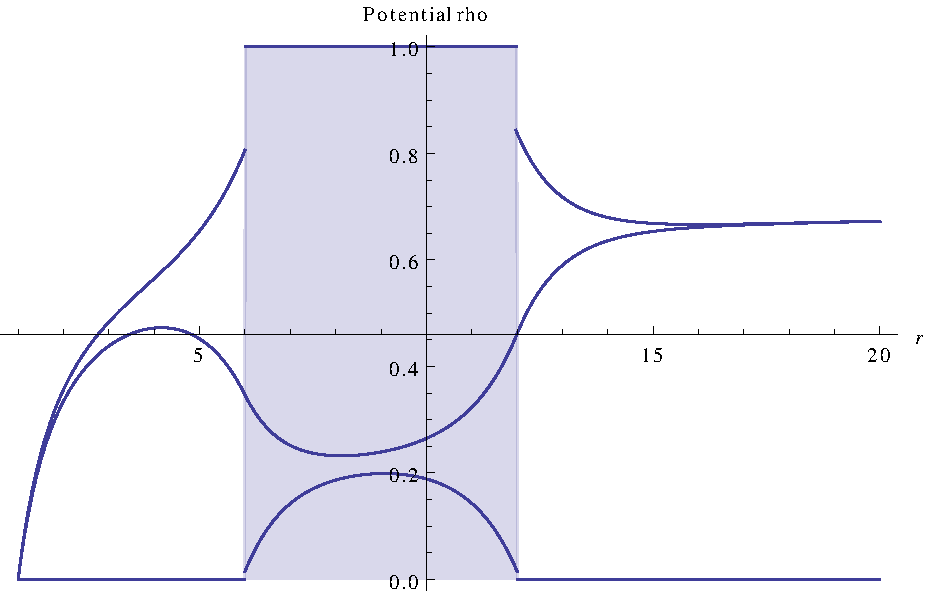
\includegraphics[width = .9 \textwidth]{plots/rho.pdf}
    \caption{Density Profiles for fluctuating repulsive potential}
    \label{fig:rho}
\end{figure}
In the following we will set $R_s = 1$ and give all other length scales relative to it.
\newpage
\subsection{Reaction Rates}
The calculation of the reaction rate as outlined in section \ref{Rates} leads to the following expression. The index of $\alpha_2$ will be omitted for reasons of convenience.
\begin{align}
    \frac{K}{K_{Debye}} &= \frac{F_1}{F_2}
    \label{two_state_rate}
\end{align}
$F_1$ and $F_2$ denote the following expressions:
\begin{align*}
    F_1 =& 2 \left(a \left(\alpha-5 b \alpha^2\right)+b \alpha-1\right) e^{2 \alpha (a+b)+u}-2 (a \alpha+1) (b \alpha-1) e^{2 (b+1) \alpha+u}-4 b \alpha (b \alpha+1) e^{3 a \alpha+b \alpha+u} \\
    &+2 b \alpha (b \alpha+1) e^{3 a \alpha+b \alpha+2 u}+4 b \alpha (b \alpha+1) e^{\alpha (a+b+2)+u}-2 b \alpha (b \alpha+1) e^{\alpha (a+b+2)+2 u} \\
    &-2 (a \alpha-1) (b \alpha+1) e^{4 a \alpha+u}+(a \alpha-1) (b \alpha+1) e^{4 a \alpha+2 u}-2 (a \alpha+1) (b \alpha+1) e^{2 (a+1) \alpha+u} \\
    &-(a \alpha+1) (b \alpha+1) e^{2 (b \alpha+u+\alpha)}-(3 a \alpha-1) (b \alpha+1) e^{2 (\alpha (a+b)+u)} \\
    &+(3 a \alpha+1) (b \alpha+1) e^{2 (a \alpha+u+\alpha)}-2 b \alpha (b \alpha+1) e^{\alpha (a+b+2)}+2 b \alpha (b \alpha+1) e^{\alpha (3 a+b)} \\
    &+e^{4 a \alpha} (a \alpha-1) (b \alpha+1)-e^{2 (a+1) \alpha} (a \alpha-1) (b \alpha+1)+(a \alpha+1) e^{2 (b+1) \alpha} (3 b \alpha-1) \\
    &-(a \alpha+1) (3 b \alpha-1) e^{2 \alpha (a+b)} \\
    F_2 =& -4 \alpha \left(a^2 \alpha-a \alpha+a-b \alpha-2\right) e^{\alpha (a+b+2)+u}+2 \alpha \left(a^2 \alpha-a \alpha+a-b \alpha-2\right) e^{\alpha (a+b+2)+2 u} \\
    &-4 \alpha \left(a^2 \alpha-a (\alpha+1)+b \alpha+2\right) e^{3 a \alpha+b \alpha+u}+2 \alpha \left(a^2 \alpha-a (\alpha+1)+b \alpha+2\right) e^{3 a \alpha+b \alpha+2 u} \\
    &+2 \alpha e^{\alpha (a+b+2)} \left(a^2 \alpha-a \alpha+a-b \alpha-2\right)+2 \alpha e^{\alpha (3 a+b)} \left(a^2 \alpha-a (\alpha+1)+b \alpha+2\right) \\
    &-\left(3 \alpha^2 (a (b-2)+2 b)+\alpha (a-3 b+4)-1\right) e^{2 (\alpha (a+b)+u)} \\
    &-2 \left(\alpha^2 (a (5 b+2)-2 b)+\alpha (a+b-4)+1\right) e^{2 \alpha (a+b)+u} \\
    &+2 (a \alpha+1) ((b-2) \alpha+1) e^{2 (b+1) \alpha+u}+2 ((a-2) \alpha-1) (b \alpha+1) e^{2 (a+1) \alpha+u} \\
    &-2 (a \alpha-1) (b \alpha+1) e^{4 a \alpha+u}+(a \alpha-1) (b \alpha+1) e^{4 a \alpha+2 u}+((a+2) \alpha+1) (b \alpha+1) e^{2 (a \alpha+u+\alpha)} \\
    &-(a \alpha+1) ((3 b-2) \alpha+1) e^{2 (b \alpha+u+\alpha)}-e^{2 \alpha (a+b)} \left(\alpha^2 (a (3 b+2)-2 b)+\alpha (-3 a+b+4)-1\right) \\
    &+e^{4 a \alpha} (a \alpha-1) (b \alpha+1)-e^{2 (a+1) \alpha} ((3 a-2) \alpha-1) (b \alpha+1)+(a \alpha+1) e^{2 (b+1) \alpha} ((b+2) \alpha-1)
\end{align*}
Sadly, this form of the solution does not tell us very much about the behaviour of the system. For a first impression, we will give some plots of the reaction rate vs. the persistence length of the solution using the parameters given above if not stated differently.\\
\begin{minipage}[t]{0.7 \textwidth}
    \begin{figure}[H]
        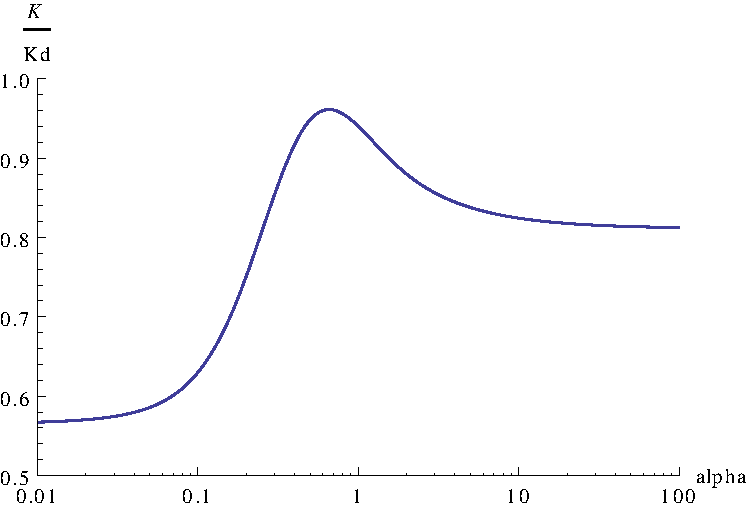
\includegraphics[width = 1 \textwidth]{plots/rate1.pdf}
    \caption{Reaction rate vs. switching rate for repulsive barrier}
    \end{figure}
\end{minipage}\begin{minipage}[t]{0.3 \textwidth}
The plot on the left shows the reaction rate relative to the reaction rate of the ungated Debye problem for a fluctuating potential barrier of hight $[U_1 = 0, U_2 = 4]$. It is obvious that it shows some sort of resonant behaviour. The reaction rate converges to some constant, finite values lower than the ungated rate and is maximised by a certain ratio of switching rate and diffusion constant. For certain parameters the rate at its maximum is even higher higher than the rate of the ungated problem.
\end{minipage}
\par
\begin{minipage}[t]{0.7 \textwidth}
    \begin{figure}[H]
        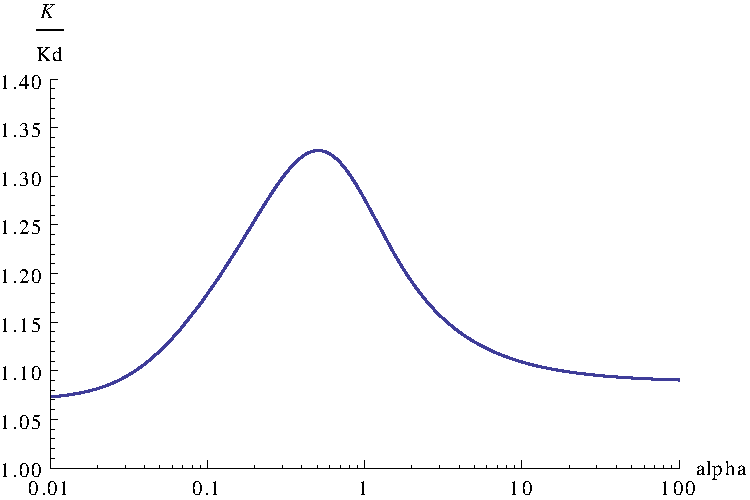
\includegraphics[width = 1 \textwidth]{plots/rate2.pdf}
    \caption{Reaction rate vs. switching rate for attractive barrier}
    \end{figure}
\end{minipage}\begin{minipage}[t]{0.3 \textwidth}
This plot shows the quotient of the reaction rates of the gated and the ungated Debye problem for an attractive fluctuating potential barrier of hight $[U_1 = 0, U_2 = -4]$. Under these conditions the reaction rate of the gated problem is always higher than the one of the ungated problem. Similar to the behaviour emerging from a repulsive barrier the rate is maximised at a certain ratio of switching rate and diffusion constant. The reaction rate at the maximum is
thereby\end{minipage}
considerably higher than at the limiting cases for very fast and very slow switching of the barrier. Comparing the repulsive barrier and the attractive barrier setting it is apparent, that the limiting cases for $\gamma/D \rightarrow 0$ and $\gamma/D \rightarrow \infty$ do differ considerably in the first case whilst in the second they do not. \par
Next we investigate if this kind of resonant activation does always occur or only for certain parameters. Therefore we calculate approximate expressions for the limiting behaviour of the reaction rate.
\subsection{Limit of $\alpha >> 1$}
To find the behaviour in the limit of $\alpha >>1$ we take a closer look at the different exponents that occur in the numerator and denominator of equation \eqref{two_state_rate}. Namely
\begin{align}
& e_1 = (3a+b)\alpha \nonumber \\
& e_2 = (2+2b)\alpha \nonumber \\
& e_3 = (2+a+b)\alpha \nonumber \\
& e_4 = 4a\alpha \nonumber \\
& e_5 = (2+2b)\alpha \nonumber \\
& e_6 = (2a+2b)\alpha
\end{align}
Using the fact that $b > a > 1$ we find that for $\alpha >>1$ the terms containing $e_6$ will dominate all others. Therefore numerator and denominator can be reduced to
\begin{align*}
    F_1' =& ( 1 + a \alpha + e^u (-1 + 3 a \alpha)) (-1 + 3 b \alpha + e^u (1 + b \alpha))\\
    F_2' =& (-1 + (4 - 3 a + b) \alpha + (2 a - 2 b + 3 a b) \alpha^2 + e^{2 u} (-1 + (4 + a - 3 b) \alpha \\
          &+ 3 (a (-2 + b) + 2 b) \alpha^2) + 2 e^u (1 + (-4 + a + b) \alpha + (2 a - 2 b + 5 a b) \alpha^2))
\end{align*}
If then again only linear and quadratic terms in $\alpha$ are collected the expression reduces to 
\begin{align}
    \frac{K}{K_{Debye}} \approx &a \left(3 e^u+1\right) \left(e^u (b x+1)+3 b x-1\right)-b \left(2 e^u+e^{2 u}-3\right) / \nonumber \\
                          &\left\{a \left(e^{2 u} (3 (b-2) x+1)+2 e^u ((5 b+2) x+1)+3 b x+2 x-3\right) \right.  \nonumber \\
                          & \left. +\left(e^u-1\right) \left(b \left(3 e^u+1\right) (2 x-1)+4 \left(e^u-1\right)\right) \right\}
    \label{kla}
\end{align}
and in the actual limit we obtain 
\begin{equation}
    \lim_{\alpha \rightarrow \infty} \frac{K}{K_{Debye}} = \frac{a b \left(e^u+3\right)}{a \left(b \left(e^u+3\right)-2 e^u+2\right)+2 b \left(e^u-1\right)}
    \label{kliminfa}
\end{equation}
\subsection{Limit of $\alpha << 1$}
To find the behaviour of the system for small $\alpha$ it proves to be sufficient to do a Taylor expansion around $\alpha_0 = 0$ to obtain
\begin{equation}
    \frac{K}{K_{Debue}} \approx \frac{\left(e^u-1\right)^2  (a-b)^2}{4 \left(a \left(b-e^u+1\right)+b \left(e^u-1\right)\right)^2} \alpha+\frac{a \left(-2 b+e^u-1\right)+b \left(1-e^u\right)}{2 \left(a \left(-b+e^u-1\right)+b \left(1-e^u\right)\right)}.
    \label{ksa}
\end{equation}
In the limit $\alpha \rightarrow 0$ then holds
\begin{equation}
    \lim_{\alpha \rightarrow 0} \frac{K}{K_{Debye}} = \frac{a \left(-2 b+e^u-1\right)+b \left(-e^u\right)+b}{2 \left(a \left(-b+e^u-1\right)+b \left(-e^u\right)+b\right)}.
    \label{klim0a}
\end{equation}
The following plots will illustrate the above \par
\begin{minipage}[t]{0.5 \textwidth}
    \begin{figure}[H]
        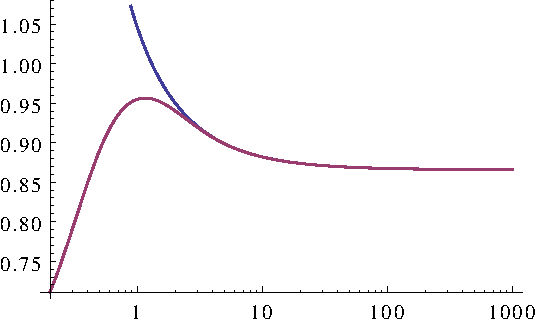
\includegraphics[width = 1 \textwidth]{plots/largelimit.pdf}
    \caption{Limit of $\alpha >>1$}
    \end{figure}
\end{minipage}\begin{minipage}[t]{0.49 \textwidth}
    \begin{figure}[H]
        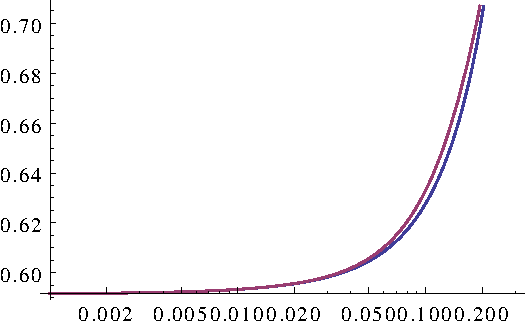
\includegraphics[width = 1 \textwidth]{plots/smalllimit.pdf}
    \caption{Limit of $\alpha <<1$}
    \end{figure}
\end{minipage}
\begin{figure}[H]
    \centering
    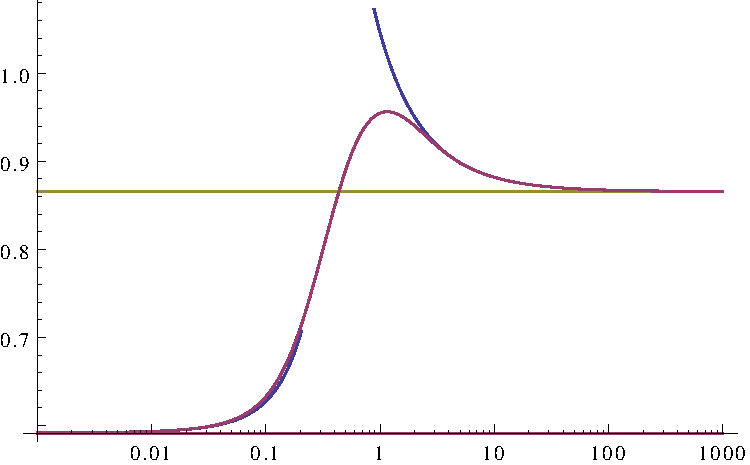
\includegraphics[width = 1 \textwidth]{plots/bothlimits.pdf}
    \caption{Limiting behaviour of Reaction Rate}
    \label{fig:rrlimit}
\end{figure}
So it seems the above calculations were correct up to this point. To prove that resonant activation always occurs it still has to be shown that the slope of the fast and slow switching limits both remain positive for all $a,b,u$. (Plotting strongly suggests it)
